\documentclass[9 pt]{beamer}




%%%%FONT
\usepackage[scaled]{helvet}
%\usepackage{times}

%%%%BACKGROUND SHADING
\setbeamertemplate{background canvas}[vertical shading][bottom=white,top=black!30]

%%%%THEMES
\usetheme{Warsaw}
\usecolortheme{seagull}
%\usetheme{Madrid}
%\usetheme{Pittsburgh}
%\usetheme{Montpellier}
%\usetheme{default}


%%%NAVIGATION, lose navigation symbols
\setbeamertemplate{navigation symbols}{}

%%%%HEADERS
%\setbeamertemplate{headline}{\vspace{1cm}}
%\setbeamertemplate{headline}{}


%%%%FOOTERS
%\setbeamertemplate{footline}{}
\setbeamertemplate{footline}[page number]{}
%\setbeamertemplate{footline}[]{}




%%%BULLETS

%these together
\setbeamercolor{itemize item}{fg=black}
%\setbeamercolor{itemize subitem}{fg=black}
%\setbeamercolor{description item}{fg=black}
%
\setbeamertemplate{itemize item}{\tiny\raise1.5pt\hbox{\textbullet}}
%\setbeamertemplate{itemize subitem}{\tiny\raise1.5pt\hbox{\textbullet}}


%these one
%\setbeamertemplate{itemize subitem}{BIOSTAT}
\setbeamertemplate{itemize subitem}{$\cdot$}

%\setbeamertemplate{itemize item}{\huge $\cdot$}




%%%%%SIZE
%\setbeamersize{text margin left=2cm}
%\setbeamersize{text margin top=0cm}







%%%%HYPERLINKS
\hypersetup{
    colorlinks,%
    citecolor=blue,%
    filecolor=green,%
    linkcolor=black,%
    urlcolor=red
}


%%%PACKAGES
\usepackage{color}
\usepackage{graphicx,amsfonts,cite,bm}
\usepackage{amsmath}
\usepackage{hyperref}
\usepackage{marvosym}
\usepackage{wrapfig}


%%%%CHANGE MATH FONT
\usefonttheme[onlymath]{serif}



%%%%WHAT DO THESE DO???
\usepackage[english]{babel}
\usepackage[latin1]{inputenc}
\usepackage[T1]{fontenc}




%%%%%% TIKZ
\usepackage{tikz}
\usetikzlibrary{arrows}

\usetikzlibrary{decorations.pathmorphing} % noisy shapes
\usetikzlibrary{positioning}
\usetikzlibrary{fit}					% fitting shapes to coordinates
\usetikzlibrary{backgrounds}	% drawing the background after the foreground
\usetikzlibrary{shapes,snakes,calendar,matrix,backgrounds,folding}


%%%%NEW COMMANDS
\newcommand{\beqa}{\begin{eqnarray*}}
\newcommand{\eeqa}{\end{eqnarray*}}
\newcommand{\beqn}{\begin{eqnarray}}
\newcommand{\eeqn}{\end{eqnarray}}
\newcommand{\be}{\begin{enumerate}}
\newcommand{\ee}{\end{enumerate}}
\newcommand{\bi}{\begin{itemize}}
\newcommand{\ei}{\end{itemize}}
\newcommand{\beq}{\begin{equation}}
\newcommand{\eeq}{\end{equation}}
\newcommand{\es}[1]{\begin{equation*}\begin{split} #1 \end{split} \end{equation*}}
\newcommand{\ilist}[1]{\bi \item #1 \ei}
\def\xii{\mathbf{x}^{(i)}}
\def\tii{\mathbf{t}^{(i)}}

\linespread{1.1}

\title[Thickness Analysis]{Simulation Study of Automated Thickness Analyzing Machine (ATAM)}
\author[YUE \& FISHER]{Chen Yue \& Aaron Fisher}
\institute[JHU Biostatictics]{Johns Hopkins Bloomberg School of Public Health\\Department of Biostatistics}
\date{\today}

\begin{document}

\begin{frame}
\titlepage
\end{frame}

\section*{Intro}
\begin{frame}
\frametitle{Background and Motivation}
\begin{enumerate}

\item<2-| alert@2> Several diseases have been found to be related to white matter loss in brain, such as Autism (Vidal 2006) and ADHD (Luders 2009). Here, we measure white matter loss based the thickness of the mid-sagittal slice of the corpus callosum (CC), the largest white matter structure in brain.\vspace{.3cm}

\item<3-| alert@3> Our objective: To analyze the link between white matter thickness along the CC, and Expanded Disability Status Scale (EDSS) score in patients with multiple sclerosis (MS). Specifically, if there are regions of the CC that are predictive of EDSS score, we want to find out where they are. \vspace{.3cm}

\item<4-| alert@4> Today we'll present a simulation study on our proposed method.
\end{enumerate}
\end{frame}

\begin{frame}
\frametitle{Background and Motivation}
\begin{figure}[ht]
\caption{CC 3D rendering and mid-sagittal slice}
\centering
\begin{minipage}[b]{.45\linewidth}
\centering
\scalebox{0.28}[0.29]{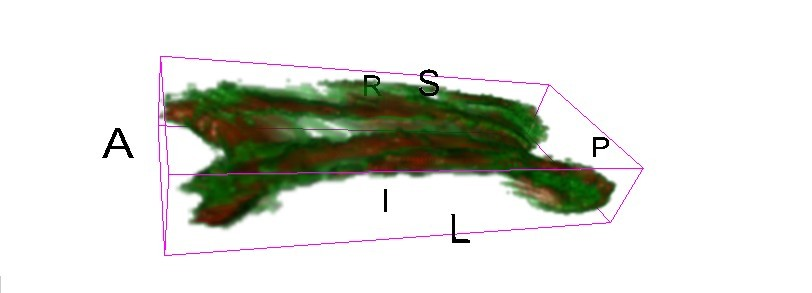
\includegraphics{pics/corpusA5.jpg}}
\end{minipage}
\begin{minipage}[b]{.45\linewidth}
\hspace{-0.2cm}
\centering
\scalebox{0.35}[0.26]{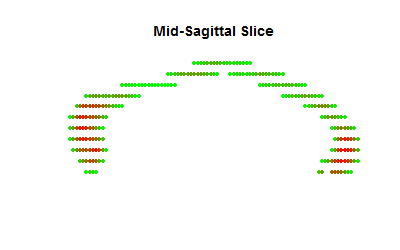
\includegraphics{pics/corpusA3.png}}
\end{minipage}
\end{figure}
Color indicates corresponding Fractional Anisotropy (FA) value.
\end{frame}

\begin{frame}
\frametitle{Pipeline}
\begin{enumerate}
\item<2-| alert@2> Obtain the center curve (principal curve) of the target data cloud.
\item<3-| alert@3> Measure the thickness.
\item<4-| alert@4> Regress the thickness function on a scalar outcome.
\item<5-| alert@5> Hypothesis testing.

%Awesome
\end{enumerate}
\end{frame}

\begin{frame}
\frametitle{Simulation Settings}
\onslide<2-| alert@2>
We first generate outcomes ($Y_i$) and shapes for each individual such that the outcome is correlated with thickness along specific regions of the principle curve.

\bi
\item<3-| alert@3>Case 1:Thickness of image$_i$ near the end points is related to $Y_i$.
\onslide<3->
\begin{figure}[!th]
\centering
\scalebox{0.2}{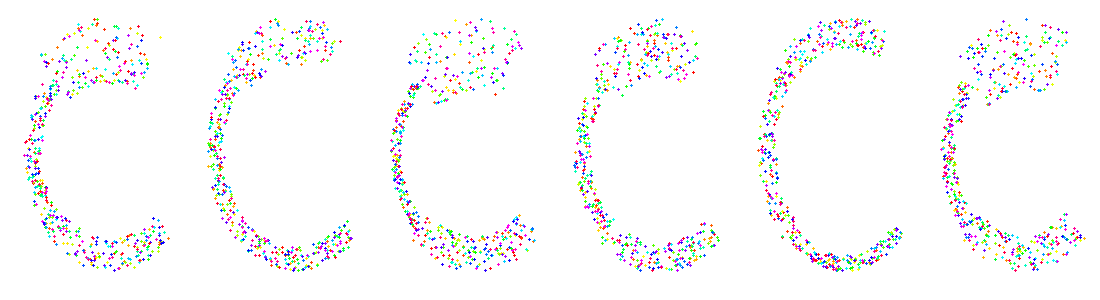
\includegraphics{pics/Simulation_C.png}}
\end{figure}\

\item<4-| alert@4> Case 2: Thickness of image$_i$ in the vertical bar is related to $Y_i$.
\onslide<4->
\begin{figure}[!th]
\centering
\scalebox{0.2}{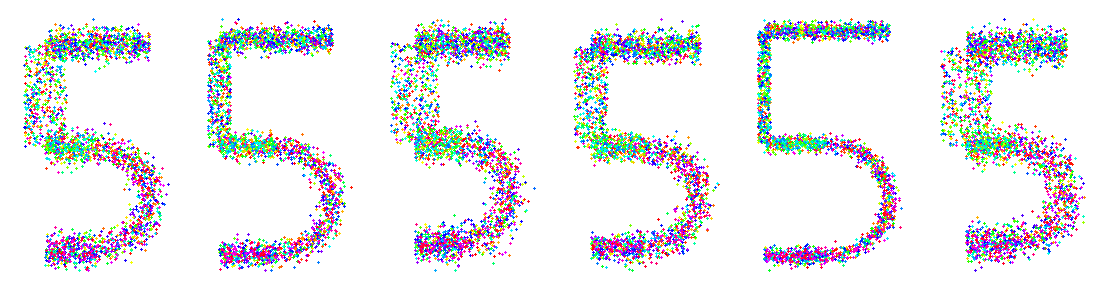
\includegraphics{pics/Simulation_5.png}}
\end{figure}
\ei
%The gray background goes really well with these colorful pictures!
\end{frame}


\begin{frame}
\frametitle{Principal curve fitting result}
\begin{figure}[ht]
\centering
\scalebox{0.27}{\includegraphics{pics/Pcurve_C.png}}
\scalebox{0.27}{\includegraphics{pics/Pcurve_5.png}}
\end{figure}
\end{frame}

\begin{frame}
\frametitle{Obtaining Thickness along the principal curve}
\begin{itemize}
\item<2-| alert@2> $\text{Thick}^*(t)=\text{Quantile}\big(\{2\times \text{dist}_{t_{j}},\big||t_{j}-t|\le.02\},\ 0.95\big)$.
\item<3-| alert@3> Fit a smooth spline across all $\text{Thick}^*(t)$.
\end{itemize}
\onslide<4->
\begin{figure}[ht]
\begin{minipage}[b]{0.45\linewidth}
\centering
\scalebox{0.27}{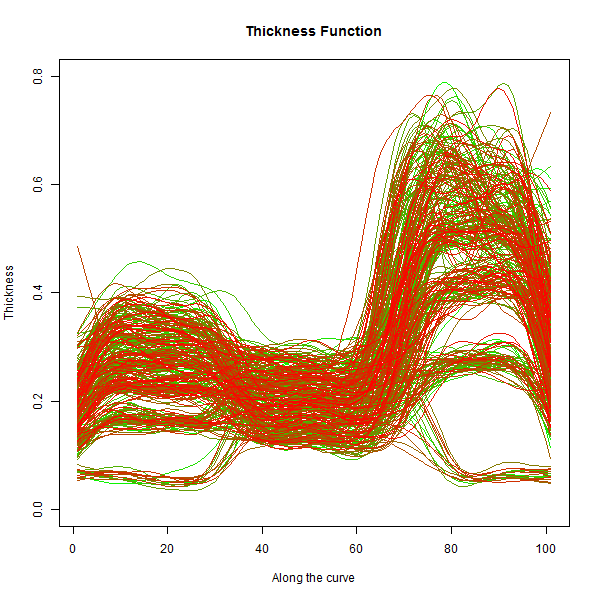
\includegraphics{pics/thickness.png}}
\end{minipage}
\begin{minipage}[b]{0.45\linewidth}
\centering
\scalebox{0.27}{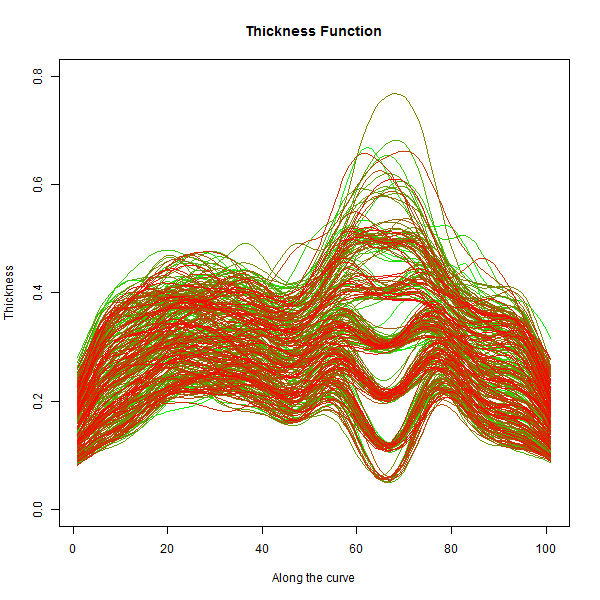
\includegraphics{pics/thickness2.png}}
\end{minipage}
\end{figure}
\end{frame}


\section*{Regression}
%%%%%%%%%%%%%%%%%%%%%%%%%%%%%%%%%%%%%%%%%%%%%%%%%
%%%%%%%%%%%%%%%%%%%%%%%%%%%%%%%%%%%%%%%%%%%%%%%%%
\begin{frame}{Regression Notation}
$Y_i$ = Outcome (simulated EDSS score) \\
$X_i(t)$= The thickness function along the track of the structure \\
$\beta(t)$ = Function representing effect of thickness on outcome, at different points.\\
$t \in [0,1]$.\\
\es{
Y_i \sim Poisson(\theta_i)\\
\theta_i =\beta_0 + \int_0^1 X_i(t)\beta(t) dt \\
}

We assume that $\beta(t)$ is a smooth function.\footnote{(Crainiceanu and Goldsmith 2010; Brezger, Kneib, and Lang 2005; Lang and Brezger 2004; Goldsmith, Feder, Crainiceanu, Caffo, and Reich, 2010)}

\end{frame}
%%%%%%%%%%%%%%%%%%%%%%%%%%%%%%%%%%%%%%%%%%%%%%%%%
%%%%%%%%%%%%%%%%%%%%%%%%%%%%%%%%%%%%%%%%%%%%%%%%%




\section*{Testing}

%%%%%%%%%%%%%%%%%%%%%%%%%%%%%%%%%%%%%%%%%%%%%%%%%
%%%%%%%%%%%%%%%%%%%%%%%%%%%%%%%%%%%%%%%%%%%%%%%%%
\begin{frame}{Pointwise \& Joint Credible Intervals - C Shape}

\begin{center}

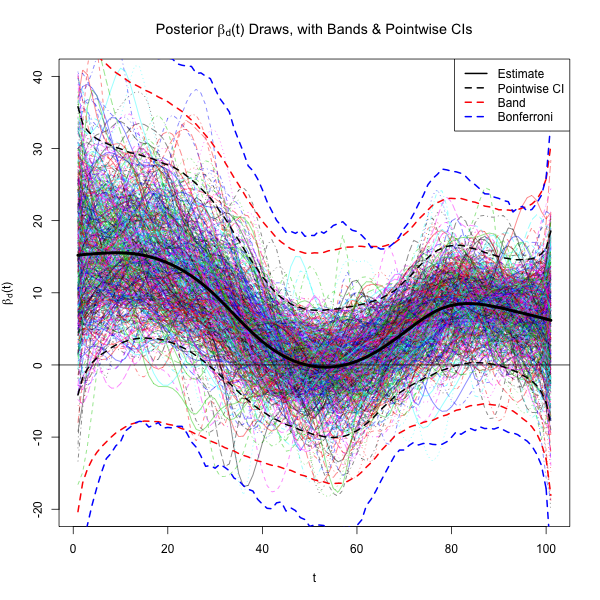
\includegraphics[scale=.37]{pics/Figure_Bands_C_Shape_12-19-12_bonf.png}

\end{center}
\end{frame}
%%%%%%%%%%%%%%%%%%%%%%%%%%%%%%%%%%%%%%%%%%%%%%%%%
%%%%%%%%%%%%%%%%%%%%%%%%%%%%%%%%%%%%%%%%%%%%%%%%%


%%%%%%%%%%%%%%%%%%%%%%%%%%%%%%%%%%%%%%%%%%%%%%%%%
%%%%%%%%%%%%%%%%%%%%%%%%%%%%%%%%%%%%%%%%%%%%%%%%%
\begin{frame}{Pointwise \& Joint Credible Intervals - 5 Shape}

\begin{center}

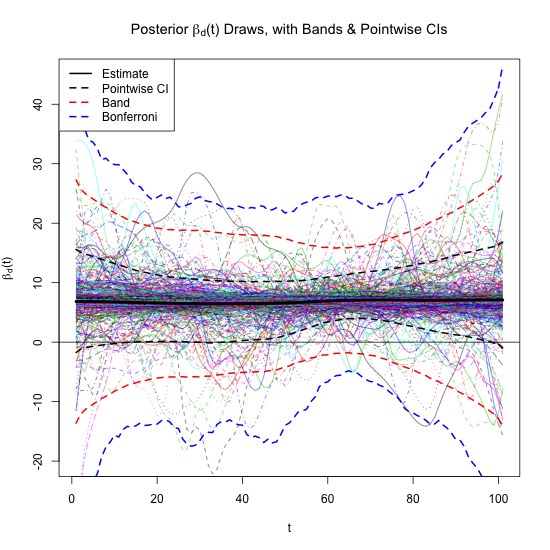
\includegraphics[scale=.37]{pics/Figure_Bands_5_Shape_12-19-12_bonf.png}

\end{center}
\end{frame}
%%%%%%%%%%%%%%%%%%%%%%%%%%%%%%%%%%%%%%%%%%%%%%%%%
%%%%%%%%%%%%%%%%%%%%%%%%%%%%%%%%%%%%%%%%%%%%%%%%%

\begin{frame}
\frametitle{Back Mapping}
\begin{figure}[ht]
\centering
\scalebox{0.27}{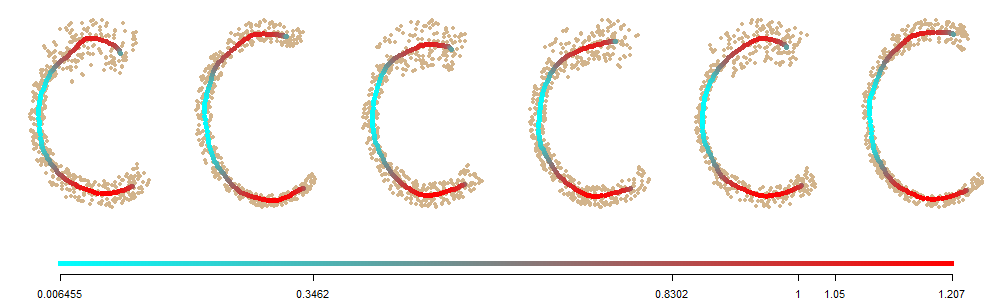
\includegraphics{pics/final_C.png}}
\scalebox{0.27}{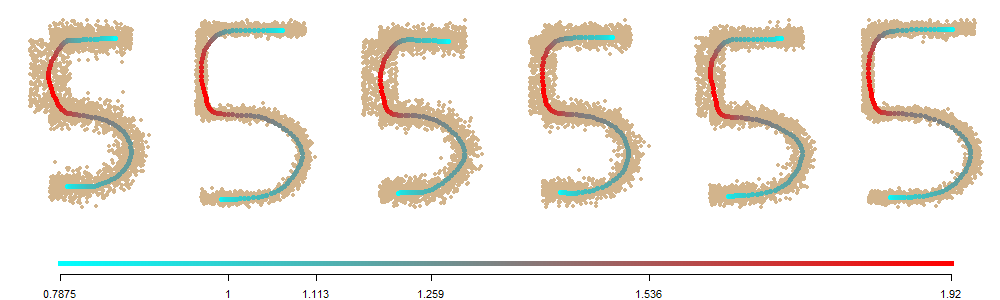
\includegraphics{pics/final_five.png}}
\end{figure}
\begin{itemize}
\item<2-| alert@2> Color indicates value $\frac{\hat{\beta}(t)}{\frac{1}{2}\text{Width}_{CI}(t)}$
\end{itemize}
\end{frame}
%%%%%%%%%%%%%%%%%%%%%%%%%%%%%%%%%%%%%%%%%%%%%%%%%
%%%%%%%%%%%%%%%%%%%%%%%%%%%%%%%%%%%%%%%%%%%%%%%%%
\begin{frame}{Discussion}
\bi
\item<1-| alert@1> The joint CI never rises above zero, but the pointwise CI does at several points. These points could be the subject of future tests, if these were real data. 
\item<2-| alert@2> Principle curve procedure sometimes doesn't work so well at the end points, if they are especially thick.
\item<2-| alert@2> Results are slightly sensitive to level of detail allowed for modelling $\beta(t)$.
\item<3-| alert@3> Currently working on an improved simulation dataset, based on a data generating process that more closely matches our real world assumptions.
\ei
\end{frame}

\begin{frame}
\frametitle{Acknowledgement}
{\bf\it Thanks to Dr. Crainiceanu, C., Gellar, J., Caffo, B., and Huang, L. for their help.}\\
\smallskip

{\bf\it Thanks for your time and attention!}
\end{frame}
\end{document}
%%%%%%%%%%%%%%%%%%%%%%%%%%%%%%%%%%%%%%%%%%%%%%%%%
%%%%%%%%%%%%%%%%%%%%%%%%%%%%%%%%%%%%%%%%%%%%%%%%%
